\section{Deformation by pivotal corridors}\label{def:section}

We now introduce a deformation of connection probabilities.  It penalizes a
connection whenever that connection must traverse an isolated open corridor.
The penalty is calibrated by a random-walk weight.  Consequently its effect
on the operator norm is small, whereas its effect on the susceptibility can
be estimated from the two ends of the corridor.

Throughout this section fix
\[
 \pc/2\le p<\pc,\qquad q=1-p,\qquad k\in\N,\quad k\ge3.
\]
Only the deformation parameter $t\ge0$ varies.  Write
\[
 T_0=T_p,\qquad m_0=\norm{T_0},\qquad
 \chi_0=\chi(p),\qquad \chi_0^+=\max_x\E_p|C_x|,
 \qquad c_\sigma=(\min_i\sigma_i)^{-1}.
\]
The walk kernel $P$, its norm $\rho<1$, and the type weights $\sigma_i$
are as in \cref{pre:mass-transport,pre:walk}.  All constants in this section depend only on
the graph, unless otherwise indicated.  In particular, their values are
uniform in the displayed range of $p$.

\begin{definition}[Templates and weighted connections]\label{def:templates}
A raw path is a $k$-step path $w=(w_0,\ldots,w_k)$ of $P$, including possible
holding steps.  Its base, endpoint, and probability are
\[
 u=w_0,\qquad v=w_k,\qquad
 \mu_u(w)=\prod_{i=0}^{k-1}P(w_i,w_{i+1}).
\]
Chronological loop erasure, with holding steps removed, gives a simple path
$\gamma_w$ from $u$ to $v$; write $\ell_w$ for its length and $I_w$ for its
internal vertices.  Retain $w$ as a \emph{template} precisely when
$\ell_w\ge3$.  The \emph{blockers} of a template $w$ are all edges incident to
$I_w$ that are not edges of $\gamma_w$; write $b_w$ for their number.  Give
this template the weight
\[
 c(w)=\mu_u(w)p^{-\ell_w}q^{-b_w}.
\]
Different raw paths remain different templates even if they have the same
loop erasure.

For an induced domain $D$, a template is eligible if $\gamma_w\subset D$.
Its raw path need not lie in $D$.  Its weight is always the full-graph weight
$c(w)$ just defined.  A blocker absent from the induced graph on $D$ counts
as closed.

If $x,y\in D$ are connected, let $N^D_{xy}$ be the sum of $c(w)$ over
eligible templates for which every edge of $\gamma_w$ is open and pivotal
for $x\leftrightarrow y$ in $D$, and every blocker is closed or absent.
Here an open edge is pivotal when closing it destroys this connection.
Set $N^D_{xy}=0$ on disconnection, and define
\[
 \begin{split}
 W_t^D(x,y)&=\one_{\{x\leftrightarrow y\text{ in }D\}}
                    e^{-tN^D_{xy}},\\
 X_t^D(x)&=\sum_{y\in D}W_t^D(x,y),\qquad
 s_t^D(x)=\E_p X_t^D(x).
 \end{split}
\]
Connections and potentials with a terminal outside $D$ are zero.
For $x\in D$, $W_t^D(x,x)=1$.  In the full graph put
\[
 T_t(x,y)=\E_pW_t^V(x,y),\qquad
 \chi_t=[s_t^V(o)],\qquad m_t=\norm{T_t}.
\]
\end{definition}

The fixed weights and the convention for absent blockers will allow us to
compare different domains without changing the deformation.

\begin{lemma}[Basic bounds and monotonicity]\label{def:basic}
There is a fixed $C>0$ such that, with $c_k=e^{Ck}$,
\begin{equation}\label{def:edge-weight}
 \sum_{w:\,e\in E(\gamma_w)}c(w)\le c_k/k
 \quad\text{for every edge }e.
\end{equation}
On a connection in a finite cluster,
$N^D_{xy}\le c_k|C_x^D|$.
For fixed $t$, $W_t^D(x,y)$ is increasing under edge openings and under
domain enlargement, using restriction of the same configuration.
The kernel $T_t$ is invariant, symmetric, and entrywise between zero and
$T_0$, and
\begin{equation}\label{def:row-norm}
 m_t\le\sup_x s_t^V(x)\le c_\sigma\chi_t.
\end{equation}
The functions $T_t(x,y)$ and $s_t^D(x)$ are continuously differentiable for
$t\ge0$, with a right derivative at zero, by differentiating
$W_t^D(x,y)$ to $-N^D_{xy}W_t^D(x,y)$ under expectation and summation.
\end{lemma}

\begin{proof}
Since $\ell_w\le k$ and $b_w\le dk$, there is a fixed $B\ge1$ with
$p^{-\ell_w}q^{-b_w}\le B^k$.  For a specified edge $e$, symmetry and
stochasticity of $P$ show that the total probability, summed over all
bases, of traversing $e$ at a specified step is $1/d$.  A union bound over
the $k$ steps therefore gives
\[
 \sum_{w:\,e\in E(\gamma_w)}c(w)
 \le B^k\sum_{u}\sum_{w:\,w\text{ traverses }e}\mu_u(w)
 \le B^k k/d.
\]
Increasing $C$ proves \eqref{def:edge-weight} for every $k\ge3$.
Every counted template has all its path edges on every simple open
$x$--$y$ path.  Charge it to an edge of one such path, which has fewer than
$|C_x^D|$ edges, to obtain the asserted bound on $N^D_{xy}$.

To prove monotonicity, consider a pair already connected before an edge
opening or a domain enlargement.  Every edge of a template counted
afterward belongs to every old simple connection.  Its retained path was
therefore already eligible, open, and pivotal.  Each blocker closed or
absent afterward was closed or absent before.  Thus every template counted
afterward was counted before, with exactly the same weight.  Its total
penalty cannot increase.  A pair previously disconnected has weight zero,
so monotonicity holds for all pairs.

Symmetry in the terminals follows directly from the pivotal condition;
it does not require any reversal property of loop erasure.  Invariance and
entrywise domination are immediate, and the row and column sum bound for
operator norms gives \eqref{def:row-norm}.
Finally,
\[
 \sum_y N^D_{xy}W_t^D(x,y)\le c_k|C_x^D|^2.
\]
The right side has finite expectation by \eqref{eq:s01} and subcritical
susceptibility finiteness.  Dominated convergence proves the differentiation
and continuity assertions.  These arguments apply to infinite domains:
their clusters are almost surely finite, and the preceding bound is
uniform under finite exhaustion.  In fact, once an exhaustion of $D$
contains the entire cluster $C_x^D$, all weighted connections inside it agree with their
limiting values: boundary blockers are closed both before and after their
other endpoints enter the domain.
\end{proof}

\begin{lemma}[Corridor calibration]\label{def:calibration}
For a template $w$, let $Q_w$ be the full-graph event that the edges of
$\gamma_w$ are open and all its blockers are closed.  Put
$D_w=V\setminus I_w$.  Then $Q_w$ is independent of the percolation in
$D_w$, and
\begin{equation}\label{def:calibration-identity}
 c(w)\Prob_p(Q_w)=\mu_u(w).
\end{equation}
On $Q_w$, the template is counted for $x\leftrightarrow y$ if and only if
one of the following two exterior events occurs:
\[
 \begin{split}
 &x\in C_u^{D_w},\quad y\in C_v^{D_w},\quad
                C_u^{D_w}\ne C_v^{D_w},\\
 &x\in C_v^{D_w},\quad y\in C_u^{D_w},\quad
                C_u^{D_w}\ne C_v^{D_w}.
 \end{split}
\]
In particular, neither terminal belongs to $I_w$.
\end{lemma}

\begin{proof}
All bits specified by $Q_w$ are incident to $I_w$, and there are exactly
$\ell_w$ specified open edges and $b_w$ specified closed edges.  This proves
independence and \eqref{def:calibration-identity}.
On $Q_w$ each internal vertex has exactly the two corridor edges open.
The resulting geometry is shown in \cref{fig:corridor}.
A simple connection using every corridor edge must traverse the whole
corridor consecutively, with both terminals outside its interior.  If the
two exterior endpoint clusters coincide, there is an exterior bypass, so
the corridor edges cannot all be pivotal.  If the exterior clusters are
distinct, the corridor is their only open link, so all of its edges are
pivotal for every terminal pair in either displayed orientation.
\end{proof}

\begin{figure}[tbp]
\centering
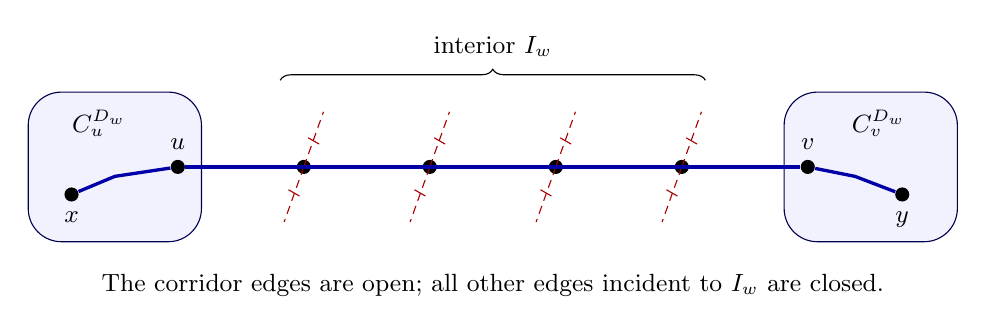
\begin{tikzpicture}[x=1cm,y=1cm,font=\small,
  dot/.style={circle,fill,inner sep=1.8pt},
  open/.style={very thick,blue!65!black},
  closed/.style={densely dashed,red!65!black}]
\fill[blue!5,rounded corners=12pt] (-1.9,-.95) rectangle (.3,.95);
\draw[blue!30!black,rounded corners=12pt] (-1.9,-.95) rectangle (.3,.95);
\fill[blue!5,rounded corners=12pt] (7.7,-.95) rectangle (9.9,.95);
\draw[blue!30!black,rounded corners=12pt] (7.7,-.95) rectangle (9.9,.95);
\node at (-1,.55) {$C_u^{D_w}$};
\node at (8.9,.55) {$C_v^{D_w}$};
\node[dot,label=below:$x$] (x) at (-1.35,-.35) {};
\node[dot,label=above:$u$] (u) at (0,0) {};
\node[dot,label=above:$v$] (v) at (8,0) {};
\node[dot,label=below:$y$] (y) at (9.2,-.35) {};
\draw[open] (x)--(-.8,-.12)--(u);
\draw[open] (v)--(8.6,-.12)--(y);
\foreach \q in {1.6,3.2,4.8,6.4}{
  \node[dot] at (\q,0) {};
  \draw[closed] (\q,0)--(\q+.25,.7);
  \draw[closed] (\q,0)--(\q-.25,-.7);
  \draw[red!65!black] (\q+.055,.37)--(\q+.195,.29);
  \draw[red!65!black] (\q-.195,-.29)--(\q-.055,-.37);
}
\draw[open] (u)--(v);
\draw[decorate,decoration={brace,amplitude=4pt}] (1.3,1.1)--(6.7,1.1)
  node[midway,above=5pt] {interior $I_w$};
\node[align=center,text width=10.5cm] at (4,-1.5)
{The corridor edges are open; all other edges incident to $I_w$ are closed.};
\end{tikzpicture}
\caption{A forced corridor and its two exterior legs. On the event that
the entire corridor is pivotal for $x\leftrightarrow y$, its endpoints
belong to distinct clusters in $D_w=V\setminus I_w$. The event $Q_w$
fixes only bits incident to $I_w$ and is independent of the exterior
percolation.
Dashed stubs represent closed blocker edges; they are schematic.}
\label{fig:corridor}
\end{figure}


\begin{proposition}[Small change of operator norm]\label{def:norm}
For every $t\ge0$,
\begin{equation}\label{eq:s27}
 0\le T_0-T_t\le 2t\,T_0P^kT_0\quad\text{entrywise},\qquad
 m_t\ge m_0-2t\rho^km_0^2.
\end{equation}
\end{proposition}

\begin{proof}
Expand $-\partial_tT_t(x,y)$ as a nonnegative sum over templates and
discard the factor $e^{-tN^V_{xy}}\le1$.  By
\cref{def:calibration}, the term for $w$ is at most
\[
 \mu_u(w)\bigl(T_0(x,u)T_0(v,y)+T_0(x,v)T_0(u,y)\bigr).
\]
Indeed the two exterior connections in each orientation belong to distinct
clusters, so BK bounds their joint probability by the product of the
corresponding full-graph connection probabilities.  Add the discarded raw
paths to this upper bound and sum over bases and endpoints.  Each orientation
gives $T_0P^kT_0$, since $P^k$ is symmetric.  Integration from zero to $t$
proves the entrywise assertion.  Domination by a nonnegative kernel gives
\[
 \norm{T_0-T_t}\le 2t\norm{T_0P^kT_0}
                  \le2t\rho^km_0^2.
\]
The triangle inequality proves the norm assertion.  In particular, no
positive-semidefiniteness assertion for $T_t$ is used.
\end{proof}

The norm estimate is one half of the comparison. We now state the
corresponding lower bound on the rate at which the averaged row sum
decreases. Let $\E_{\rm path}$ denote averaging over the type-weighted
root $u=o$ and a length-$k$ $P$-path from $u$. Denote its endpoint by
$v$, whether or not the path is retained as a template, and put
$a_3=\tr(T_0^3)$.

\begin{proposition}[Decrease of the averaged susceptibility]\label{def:decrease}
For all $t\ge0$,
\begin{equation}\label{eq:s31}
 -\chi_t'\ge e^{-tc_k}
 \left(
 \E_{\rm path}\left[
       \one_{\{\ell_w\ge3\}}s_t^{D_w}(u)s_t^{D_w}(v)\right]
       -C'(\chi_0^+)^2\rho^ka_3
 \right),
\end{equation}
where $C'>0$ depends only on $G$.
The product term is defined to be zero for discarded raw paths.
\end{proposition}

The product measures the weighted connection mass available at the
two exterior endpoints. We will prove this bound by estimating the
loss under deletion, separating the two exterior clusters, and
comparing their penalties with that of the full connection. To make the
product dominate the error, we still need paths on which both endpoint
potentials remain large. Constructing such paths is the task of the next
section.

\begin{lemma}[Deletion estimate]\label{def:deletion}
For $A\subset D$, let $\Nb[A]$ denote $A$ together with all its neighbors
in the full graph.  For every vertex $v$,
\begin{equation}\label{eq:s28}
 s_t^{D\setminus A}(v)
 \ge s_t^D(v)-\chi_0^+\sum_{z\in\Nb[A]}T_0(v,z).
\end{equation}
\end{lemma}

\begin{proof}
We first compare weighted connections in a fixed configuration.  Suppose
$W_t^D(v,y)>W_t^{D\setminus A}(v,y)$.  There was an old connection.  If
deletion destroys it, an old simple $v$--$y$ path visits $A$; this includes
the case of a deleted terminal.  Otherwise some positive-weight template
is newly counted after deletion.  Its retained path already lay in $D$ and
was open there.  The raw path and its weight have not changed, so there are
only two possible reasons it was not counted before.

First, a path edge may previously have been nonpivotal.  An old simple
connection avoiding that edge must visit $A$, since otherwise the edge
would remain nonpivotal after deletion.  Second, a blocker may previously
have been open.  Since it is now absent, it joins an internal retained-path
vertex $z\notin A$ to a vertex of $A$.  Every surviving simple connection
uses the new template path and therefore visits this
$z\in\Nb[A]$.  This second case includes a removed pendant branch: its
attachment vertex, rather than the removed vertex, lies on the connection.

The entire positive loss, which is at most one, is thus bounded by the
indicator that some old simple $v$--$y$ path visits $\Nb[A]$.  Splitting
such a path at a visited vertex $z$ gives edge-disjoint connection
witnesses from $v$ to $z$ and from $z$ to $y$.  A union bound and BK yield
\[
 \E_p\bigl(W_t^D(v,y)-W_t^{D\setminus A}(v,y)\bigr)
 \le\sum_{z\in\Nb[A]}T_0(v,z)T_0(z,y).
\]
There is no sum over penalty weights in this estimate: a single visiting
event bounds the whole loss.  Summing over $y$ proves \eqref{eq:s28}.
For infinite $A$ all sums are interpreted monotonically, with an infinite
right-hand error giving a trivial bound.
\end{proof}

\begin{lemma}[Two distinct exterior clusters]\label{def:correlation}
There is a constant $C'>0$ such that, for every induced domain $D$ and
$u,v\in D$,
\begin{equation}\label{eq:s29}
 \E_p\bigl(X_t^D(u)X_t^D(v);\ C_u^D\ne C_v^D\bigr)
 \ge s_t^D(u)s_t^D(v)-C'(\chi_0^+)^2T_0^3(u,v).
\end{equation}
The constant is independent of $D,p,k,t$.
\end{lemma}

\begin{proof}
Expose the exact finite cluster $A=C_u^D$, including every internal edge
bit and its closed boundary.  This determines $X_t^D(u)$: every counted
template has retained path in $A$, its weight is deterministic, and its
blockers leaving $A$ are closed or absent.  The edges with both endpoints
in $D\setminus A$ remain independent Bernoulli variables of parameter $p$.

For terminals in a cluster outside $A$, weighted connections before and
after deleting $A$ agree exactly.  All open paths stay in that exterior
cluster; every eligible counted retained path stays there too; the only
blockers removed were closed contacts with $A$.  Raw excursions into $A$
affect neither eligibility nor weight.  Consequently, including $v\in A$
by the zero convention,
\begin{equation}\label{def:cluster-exposure}
 \E_p\bigl(X_t^D(u)X_t^D(v);\ C_u^D\ne C_v^D\bigr)
 =\E_p\bigl[X_t^D(u)s_t^{D\setminus A}(v)\bigr].
\end{equation}
Apply \cref{def:deletion} inside this expectation and use
$X_t^D(u)\le |A|$.  For adjacent $a,z$, positive association with the event
that their edge is open gives $pT_0(v,z)\le T_0(v,a)$.  Hence
\[
 \sum_{z\in\Nb[A]}T_0(v,z)
 \le(1+d/p)\sum_{a\in A}T_0(v,a).
\]
The three-arm estimate \eqref{eq:s01}, summed over a third terminal, gives
\[
 \begin{split}
 \E_p\bigl(|A|\one_{\{a\in A\}}\bigr)
 &=\sum_y\Prob_p(u\leftrightarrow a,\ u\leftrightarrow y\text{ in }D)\\
 &\le\sum_b T_0(u,b)T_0(b,a)\sum_y T_0(b,y)
 \le\chi_0^+T_0^2(u,a).
 \end{split}
\]
The error in \eqref{def:cluster-exposure} is therefore at most
\[
 (1+d/p)(\chi_0^+)^2\sum_a T_0^2(u,a)T_0(a,v),
\]
which proves \eqref{eq:s29} with $C'=1+2d/\pc$.
\end{proof}

\begin{lemma}[Decomposition into two legs]\label{def:legs}
On $Q_w$, suppose
$x\in C_u^{D_w}$, $y\in C_v^{D_w}$, and
$C_u^{D_w}\ne C_v^{D_w}$.  Then
\begin{equation}\label{eq:s30}
 N^V_{xy}\le c_k+N^{D_w}_{xu}+N^{D_w}_{vy}.
\end{equation}
\end{lemma}

\begin{proof}
The total weight of all templates whose retained paths use any edge of
$\gamma_w$ is at most $\ell_wc_k/k\le c_k$, by
\eqref{def:edge-weight}.  Consider any remaining template counted for
$x\leftrightarrow y$.  Its retained path cannot meet $I_w$: every open edge
incident to $I_w$ is an edge of $\gamma_w$.  Its connected retained path
thus lies in one of the two distinct exterior endpoint clusters.

If it lies in the $u$ cluster, every one of its edges is pivotal for the
exterior connection $x\leftrightarrow u$.  Otherwise an exterior
$x$--$u$ path avoiding that edge, followed by the corridor and an exterior
$v$--$y$ path, would give a global $x$--$y$ connection avoiding it.  Its
blockers remain closed or absent on restriction to $D_w$.  Thus it is
counted, with the same weight, in $N^{D_w}_{xu}$.  The $v$ cluster gives
$N^{D_w}_{vy}$ in the same way.  This proves the bound.
\end{proof}

\begin{proof}[Proof of \cref{def:decrease}]
Expand the negative derivative of $\chi_t$ as the sum over the starting
terminal, the other terminal, and all counted templates.  Use the
mass-transport identity \eqref{eq:s02} to move the root from the starting
terminal to the template base.  All terms are nonnegative, so this
rearrangement is justified by Tonelli's theorem.  For each template retain
only the orientation $x\in C_u^{D_w}$, $y\in C_v^{D_w}$.
On $Q_w$ and this exterior event, \cref{def:legs} implies
\[
 W_t^V(x,y)\ge
 e^{-tc_k}W_t^{D_w}(x,u)W_t^{D_w}(v,y).
\]
Independence of $Q_w$ from the exterior and
\eqref{def:calibration-identity} replace its factor $c(w)$ by $\mu_u(w)$.
After summing over $x,y$, we obtain
\[
 -\chi_t'\ge e^{-tc_k}\E_{\rm path}\left[
 \one_{\{\ell_w\ge3\}}
 \E_p\bigl(X_t^{D_w}(u)X_t^{D_w}(v);
           C_u^{D_w}\ne C_v^{D_w}\bigr)\right].
\]
Apply \cref{def:correlation}.  For its nonnegative error kernel, adding
discarded paths only increases the average, and
\[
 \E_{\rm path}T_0^3(u,v)
 =[\sum_v P^k(o,v)T_0^3(v,o)]
 =\tr(P^kT_0^3)\le\rho^k\tr(T_0^3).
\]
The last inequality uses the positive operator $T_0^3$ and the positive
trace inequality of \cref{pre:trace} for the self-adjoint operator $P^k$.  It requires no
commutation of $P$ with $T_0$.  This proves \eqref{eq:s31}.
\end{proof}

The deletion error can be smaller at a vertex near a corridor endpoint
than at the endpoint itself. The following comparison transfers the
potential from that vertex back along a fixed path.

\begin{lemma}[Comparison along a path]\label{def:endpoint}
If a simple path in $D$ joins $b$ to $z$ and has length $l$, then
\begin{equation}\label{eq:s32}
 s_t^D(b)\ge e^{-tlc_k}p^l s_t^D(z).
\end{equation}
\end{lemma}

\begin{proof}
Let $F$ be the event that this fixed path is open.  On $F$ and on a
connection from $z$ to $y$, there is also a connection from $b$ to $y$.
Templates counted for the latter connection whose retained paths use an
edge of the fixed path have total weight at most $lc_k$, by
\eqref{def:edge-weight}.  For any other counted template, every retained
edge is pivotal for $z\leftrightarrow y$: a $z$--$y$ bypass, concatenated
with the fixed $b$--$z$ path, would otherwise give a $b$--$y$ bypass.
Its blocker condition is unchanged.  Thus, on $F$,
\[
 W_t^D(b,y)\ge e^{-tlc_k}W_t^D(z,y).
\]
Both $\one_F$ and $W_t^D(z,y)$ are increasing functions of the percolation
bits, by \cref{def:basic}.  Positive association and $\Prob_p(F)=p^l$
give
\[
 \E_pW_t^D(b,y)
 \ge e^{-tlc_k}\E_p[\one_FW_t^D(z,y)]
 \ge e^{-tlc_k}p^l\E_pW_t^D(z,y).
\]
Summation over $y$ proves \eqref{eq:s32}.
\end{proof}
